\documentclass[]{exam}
\usepackage{amssymb}
\usepackage{amsfonts}
\usepackage{amsmath}
\usepackage{amsthm}
\usepackage[top=1in, bottom=1.5in, left=1in, right=1in]{geometry}
\usepackage{tikz}
\usepackage{pgfplots}
\usepackage{empheq}
\usepackage{mathrsfs}
\checkboxchar{$\Box$}
\usepackage{graphicx}
\usepackage{caption}
\usepackage{float}
\usepackage{enumerate}
\usepackage{comment}
\usepackage{multicol}
\usepackage{color}
\usepackage{advdate}
\usepackage{gensymb}
\usetikzlibrary{arrows}
\usepackage{multirow}
\usepackage{arydshln}
\usepackage{verbatim}

\usepackage{pgfkeys,pgfcalendar}

\newcount\pgfdatecount
\newcommand{\tomorrow}{%
\pgfcalendardatetojulian{\year-\month-\day+1}{\pgfdatecount}
\pgfcalendarjuliantodate{\the\pgfdatecount}{\myyear}{\mymonth}{\myday}
\pgfcalendarmonthname{\mymonth}\space\myday,\space\myyear%
}

\newcommand{\advanceday}[1][1]{
\begingroup
\AdvanceDate[#1]
\today
\endgroup}

\newcommand{\vertex}{\node[vertex]}
\tikzstyle{vertex}=[circle, draw, inner sep=0pt, minimum size=6pt]
\usepackage{lastpage} 
\usepackage{extramarks}
\usepackage{graphicx} 
\usepackage{tikz}
\usepackage{sectsty} 
\usepackage{amsmath,amsfonts,amsthm} 
\usepackage{wrapfig, blindtext}

% Margins
\topmargin=-0.45in
\evensidemargin=0in
\oddsidemargin=0in
\textwidth=6.5in
\textheight=9.0in
\headsep=0.25in 
\numberwithin{equation}{section}
\linespread{1.1} 
\setlength\parindent{0pt} 
\setlength\answerskip{-.075in}
\setlength\answerlinelength{.5in}
\newcommand{\myitem}{\item[-]}

% HEADER AND FOOTER
\pagestyle{headandfoot}
\runningheadrule
\runningfootrule
\firstpageheader{Kutztown University}{  }{MATH 210}
\firstpageheadrule
\runningheader{P1.H1}{ }{MATH 210}
\firstpagefooter{}{}{} 
\runningfooter{}{}{Page \thepage\ of \numpages}


% TITLE PAGE
\newcommand{\assignmentname}{Phase 1 -- Homework I} % Assignment title
\newcommand{\coursetitle}{MATH 210 -- Mathematical Computing and Typesetting}
\newcommand{\duedate}{Due: Friday, February 6 by 11:59 PM on D2L} % Class/lecture time
\newcommand{\readsections}{\, } % Teacher/lecturer
\newcommand{\semester}{\, }
\title{
\vspace{2in}
\textmd{\textbf{\course:\ \assignmentname}}\\
\normalsize\vspace{0.1in}{\duedate}\\
\vspace{0.1in}\large{\textit{\instructor}}
\vspace{3in}
}
\author{\textbf{Author: \authorname}}
\date{Last Updated: \today}

\pointsinrightmargin
\bracketedpoints



\begin{document}
%%%%%%%%%%%%%%%%%%%%%%%%%%%%%%%%%%%%%%%%%%%%%%%%%%%%%
% COMPILE TITLES AND SUCH
%%%%%%%%%%%%%%%%%%%%%%%%%%%%%%%%%%%%%%%%%%%%%%%%%%%%%
\hspace{1in}\\ \vspace{.15in}


\begin{center}
\normalsize
 \fbox{\fbox{\parbox{5.5in}{
        {\bf Instructions:}  Upload the \texttt{tex} file for this document to your Overleaf project.  All solutions shall be completed on this packet by typing your solution in \LaTeX\, in the space provided.  All solutions should be detailed and should clearly demonstrate the process by which you arrived at the answer.  Submit the compiled \texttt{pdf} file to D2L by 11:59 PM on the due date below.  Submit only a single pdf file of your entire packet.  The question will also ask you to make calculations in Python.  Upload any Python files to the appropriate folder in your GitHub repository.  In this folder, a \texttt{py} file is to be submitted for each problem such that when the \texttt{py} file is executed, the output (as presented in Python) is the solution to the problem. Academic dishonesty will not be tolerated.  }}}
\end{center}

\vspace{.5cm}

\begin{center}
	\Huge\textsc{
	\assignmentname}\\[4pt]
        \Large{\textsc{\coursetitle}\\[10pt]}
        \Large{\textsc{\duedate}\\[8pt]}
        \Large{\textsc{\readsections}\\[8pt]}
\end{center}

\vspace{1cm}

%%%%%%%%%%%%%%%%%%%%%%%%%%%%%%%%%%%%%%
% Uncomment the syntax below when you type up the solutions and type 
% your name.
\begin{center}
	\large{\textsc{\textcolor{red}{Solutions by Brooks Emerick}}}
\end{center}
\vfill

%%%%%%%%%%%%%%%%%%%%%%%%%%%%%%%%%%%%%%
% Reminders:
%%%%%%%%%%%%%%%%%%%%%%%%%%%%%%%%%%%%%%
Remember to begin your \texttt{py} file with \texttt{import numpy as np} and \verb|import matplotlib.pyplot as plt|.  Also, for this assignment, you'll need \texttt{from scipy.optimize import minimize} for finding relative extrema of functions.  



% Blank Page
\clearpage

\begin{questions}
%%%%%%%%%%%%%%%%%%%%%%%%%%%%%%%%%%%%%%
% NUMBER 1 
%%%%%%%%%%%%%%%%%%%%%%%%%%%%%%%%%%%%%%
\question Define the function 
	\[ \displaystyle f(x) =  \frac{x}{30} - e^{-\frac{x}{6}}\cos(x)\]
in a Python file.  In the space below, determine the derivative function and type it, centered in math display mode.  \\

\textsc{Solution:} Using the power rule and the product rule for derivatives, we have 

\begin{align*}
	f'(x) & = \frac{1}{30} - \left( -\frac{1}{6} e^{-x/6} \cos(x) + e^{-x/6}\big(-\sin(x)\big) \right) \\ 
	& = \frac{1}{30} + \frac{1}{6}e^{-x/6}\cos(x) + e^{-x/6}\sin(x) \end{align*}


In the Python file, define the derivative function as well.  Graph both functions on the same graph.  The graph should be black, solid, and have line width 3.  The title should be \texttt{Homework 1, Plot 1}.  Use \texttt{plt.xlim} and \texttt{plt.ylim} to create a ``tight'' window, i.e., the $x$-axis should span from $-5$ to $20$ and the $y$-axis should span from the minimum value of $y$ to the maximum value of $y$.  The plot should show a legend.  Your code should save this plot as a high resolution \texttt{eps} file.  (Hint: consider the commands \texttt{np.min()} and \texttt{np.max()}.)  Include the graph in the space below.  

\textsc{Solution:} The plot from Python is given below: 

\begin{figure}[h!]
\begin{center}
	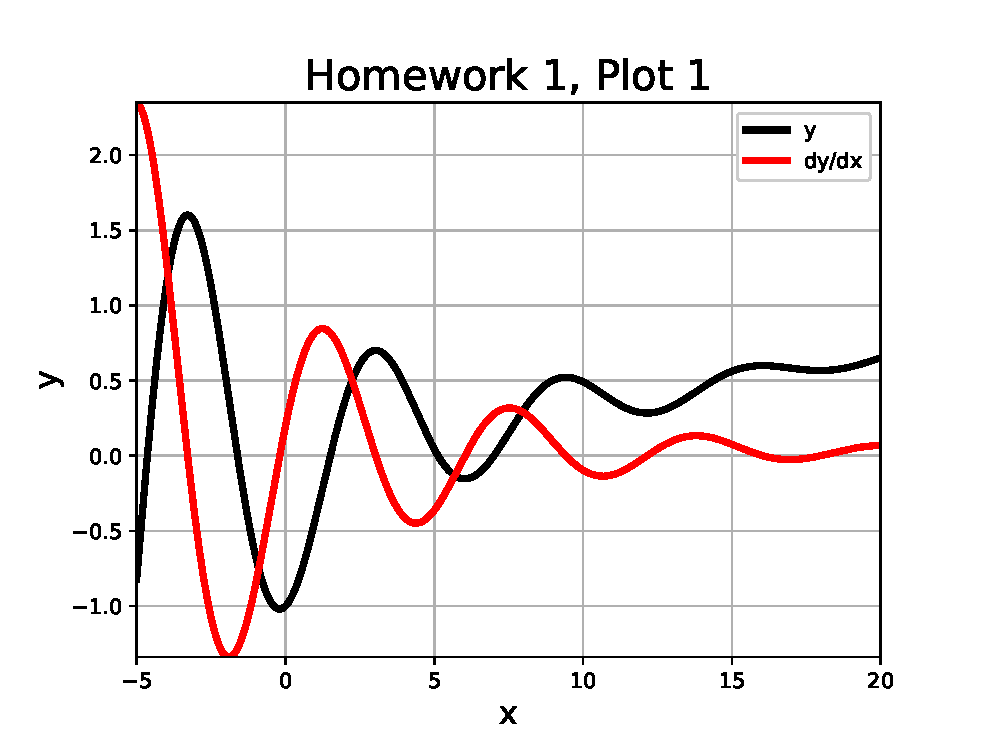
\includegraphics[width = .8\textwidth]{p1hw1_plot1.eps}
\end{center}
\caption{Plot of $f(x)$ and $f'(x)$.  }
\end{figure}

\pagebreak

%%%%%%%%%%%%%%%%%%%%%%%%%%%%%%%%%%%%%%
% NUMBER 2
%%%%%%%%%%%%%%%%%%%%%%%%%%%%%%%%%%%%%%
\question Consider the function 
\[y = x^3-7x^2+10x\]
over the interval $x\in [-1,6]$.  

\begin{parts}
	\part Determine the equation of the tangent line to this graph at $x = 1$, $x = 3$ and $x = 5$.  Type your work below explicitly showing the derivative function and the three tangent line equations. 

\textsc{Solution:} The $y$-values at each of the three points are 
\begin{align*}
y_1 & = (1)^3-7(1)^2+10(1) = 4\\ 
y_2 & = (3)^3-7(3)^2+10(3) = -6\\ 
y_3 & = (5)^3-7(5)^2+10(5) = 0\end{align*}

The derivative is given by 
\[ \frac{dy}{dx} = 3x^2 -14x + 10.\]

The slope of the tangent line at each point is given by the following: 
\begin{align*}
m_1 & = \left. \frac{dy}{dx} \right|_{x = 1} = 3(1)^2 - 14(1) + 10 = -1\\ 
m_2 & = \left. \frac{dy}{dx} \right|_{x = 3} = 3(3)^2 - 14(3) + 10 = -5\\ 
m_3 & = \left. \frac{dy}{dx} \right|_{x = 5} = 3(5)^2 - 14(5) + 10 = 15\end{align*}

Let $(x_i, y_i)$ be any point on the tangent line with slope $m_i$  to a function $y = f(x)$ at $x_i$, then the line has the following slope intercept form: 
\[ y - y_i  = m_i(x-x_i)  \qquad \Rightarrow \qquad y = m_i x + y_i - m_i x_i,\]
We note the $y$-intercept is given by $b_i = y_i - m_ix_i$: 
\begin{align*}
b_1 & = y_1 - m_1 x_1 = 4 - (-1)(1) = 5\\ 
b_2 & = y_2 - m_2 x_2 = -6 - (-5)(3) = 9\\ 
b_3 & = y_3 - m_3 x_3 = 0 - (15)(5) = -75 \end{align*}

Finally, we can write the tangent line at each point: 
\begin{align*}
\text{Tangent Line at $x = 1$:} & \qquad y = -x +5 \\ 
\text{Tangent Line at $x = 3$:} & \qquad y = -5x +9 \\ 
\text{Tangent Line at $x = 5$:} & \qquad y = 15x +75  \end{align*}

In a Python file, define $y$ and the tangent lines as functions.  Plot $y$ over the interval $[-1, 6]$ in solid black with line width 3 with title \texttt{Homework 1, Plot 2}.  Plot on this same graph the tangent lines to the curve at $x = 1$, $x = 3$, and $x = 5$ in red, green, and blue lines, respectively.  Provide a legend.  Your code should save this plot as a high resolution \texttt{eps} file. Include the graph in the space below. 

\pagebreak 

\textsc{Solution:} The plot from Python is given below: 

\begin{figure}[h!]
\begin{center}
	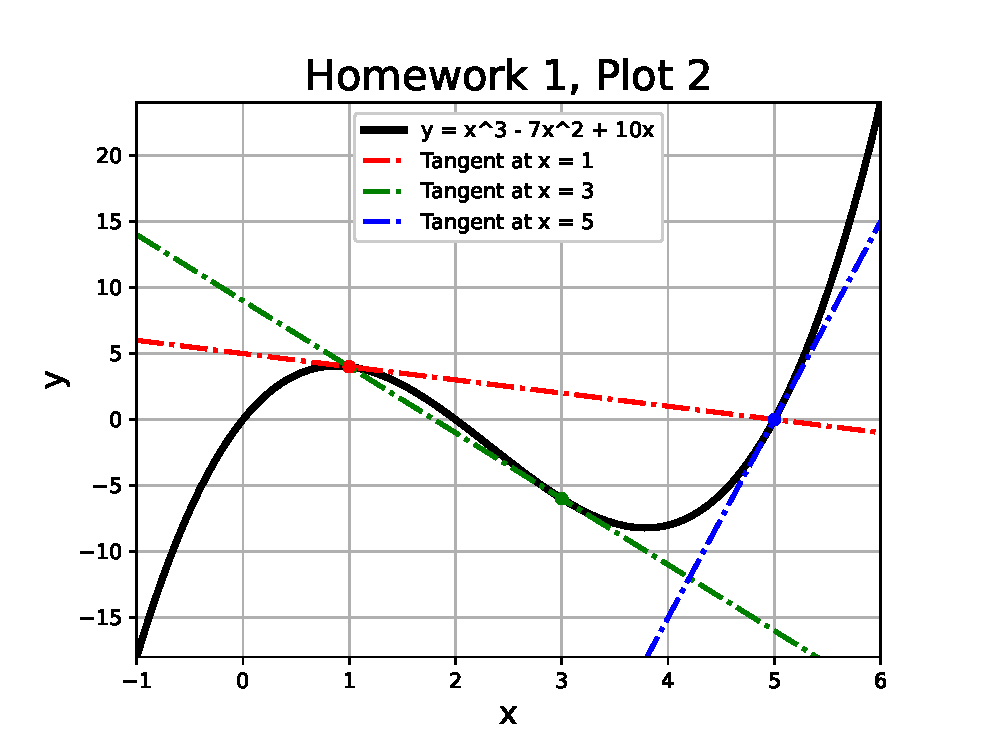
\includegraphics[width = .8\textwidth]{p1hw1_plot2.eps}
\end{center}
\caption{Plot of $y$ with the three tangent lines.  }
\end{figure}


	\part Find the exact values of the critical points of this function ($x$ value only) and type your work and solution in the space below. 
	
\textsc{Solution:}  Using the quadratic formula to solve $dy/dx = 0$, we have 
\begin{align*}
x & = \frac{-(-14) \pm \sqrt{(-14)^2 - 4(3)(10)}}{2(3)} \\ 
& = \frac{14 \pm \sqrt{196-120}}{6} \\  
& = \frac{14 \pm \sqrt{76}}{6} \\ 
& = \frac{14 \pm 2\sqrt{19}}{6} \\ 
& = \frac{7}{3} \pm \frac{\sqrt{19}}{3}\end{align*}

A numerical approximation to each critical is given by
\[ c_1 = \frac{7}{3} - \frac{\sqrt{19}}{3} \approx 0.880 \qquad \text{and} \qquad c_2 = \frac{7}{3} + \frac{\sqrt{19}}{3} \approx 3.786 \]
We note that both points are interior to the interval $[-1,6]$.  \\


In the same Python file, use \texttt{minimize} to compute both the relative minimum and maximum value of $y$ on the interval $[-1,6]$.  Report the results below to three decimals and confirm that your exact solution matches.   


\textsc{Solution:} From Python, the function \texttt{optimize.minimize} outputs 3.79 for the relative minimum and 0.88 for the relative maximum, which is consistent with the exact solution. 
\end{parts}






\end{questions}
\end{document} 
